\documentclass[11pt,letterpaper]{article}
\usepackage{graphicx, geometry, amsmath, hyperref, booktabs, xcolor, listings}
\geometry{margin=1in}
\hypersetup{colorlinks=true, linkcolor=black, citecolor=black, urlcolor=black}

\title{Measuring Authority Diffusion Before Founders Leave Open Source Projects}
\author{}
\date{}

\begin{document}
\maketitle

\begin{abstract}
Open-source projects often depend on a single founding developer, and predicting whether a project survives once that developer stops committing -- a Truck-Factor Developer Detachment, following Avelino et al. -- is an open problem: at the moment of detachment, surviving and non-surviving projects look statistically indistinguishable in size. We build and calibrate an instrument to test whether the missing signal instead lies in the trend of authority concentration in the months before departure, reimplementing Avelino et al.'s Degree-of-Authorship / Truck-Factor pipeline and adding a new pre-departure authority-diffusion measurement. The reimplementation reproduces Avelino et al.'s published statistics closely enough to trust, and a fully disclosed permutation test confirms the diffusion measurement is specific to the pre-departure window rather than a generic property of active projects -- evidence that validates the measurement instrument, not evidence that diffusion predicts survival. A calibration gate applied to our corpus shows why the causal claim cannot yet be tested: a corpus built by starting from currently famous, still-maintained repositories structurally excludes the non-surviving projects the hypothesis needs to observe, a defect no larger sample from the same source would fix. We report this paper's contribution accordingly: a validated measurement instrument, an exact accounting of its permutation-test mechanics, a formal demonstration of why the sampling frame -- not the sample size -- blocks the causal question, and a scoped, partially executed alternative data pipeline for a follow-up study that could finally test it.
\end{abstract}

\section{Introduction}

Open-source software projects routinely depend on the sustained attention of one or two people. When the developer who founded such a project stops committing, the project faces what Avelino et al. call a Truck-Factor Developer Detachment (TFDD): every developer in the project's minimal Truck-Factor set has gone silent for at least a validated twelve-month abandoner threshold [1]. Some of these projects go dark permanently; others are picked up by new maintainers and continue for years. What determines which outcome a given project has, before it happens, is the question this paper set out to answer. Avelino et al.'s own results show the obvious predictor does not work: at the TFDD snapshot itself, surviving and non-surviving projects are statistically indistinguishable in developers, commits, and files (Cohen's d = 0.13-0.26) [1]. Their finding leaves an open question -- if size at departure carries no signal, does the trend leading up to departure carry any? -- and this paper builds and rigorously calibrates the instrument needed to ask it.

We do not, in the end, answer that question empirically. This paper is a methodology and measurement contribution, not an empirical resolution of it, and we state that plainly up front rather than let it surface only in the limitations. We built a full reimplementation of Avelino et al.'s Degree-of-Authorship (DOA) / Truck-Factor / TFDD pipeline, added a new pre-departure authority-diffusion measurement -- founder commit-share and the count of distinct non-founder DOA-owners in the six to twelve months before a founder-only TFDD -- and subjected both to a two-stage calibration and robustness harness. Run on a corpus of 15 well-known GitHub repositories, the instrument reproduces Avelino et al.'s founder-only-detachment statistic within overlapping confidence intervals and shows the diffusion measurement is temporally specific to the pre-departure window rather than a generic feature of active codebases. But the corpus on which this all runs cannot test the causal claim that motivated it, and the reason is structural rather than a matter of needing more data of the same kind.

\textbf{Why the causal question is hard to test with this design.} A corpus assembled by starting from repositories that are famous and actively maintained \emph{today} -- the only kind reachable within an unauthenticated 60-request-per-hour GitHub API budget in a short execution window -- necessarily excludes almost all repositories that experienced a founder departure and then genuinely died, because a dead, obscure repository is exactly the kind of project such a candidate list would never include in the first place. This is not an underpowered sample of the right population; it is a sample of the wrong population, one where the outcome variable is conditioned on before the study even begins. A calibration gate applied to this corpus makes the argument concrete rather than rhetorical: the corpus's Truck-Factor-Detachment incidence rate is 73.3\% (11 of 15 repositories) against Avelino et al.'s published 16.3\% (315 of 1,932) -- a difference so large it is not plausibly sampling noise (two-proportion z = 5.98, exact binomial p = 1.5e-6) -- and the 18-month post-detachment survival rate among the five founder-only TFDDs this corpus contains is 100\%, against Avelino et al.'s published 40.6\% (z = 2.70, p = 0.011). Both deviations point the same direction a "famous tools that still exist" sampling frame predicts: it over-represents projects that survived whatever they went through, and it can never, no matter how many more repositories are added from the same frame, produce the non-surviving founder-only-TFDD event this paper's headline hypothesis needs to test against. Enlarging this corpus would sharpen the wrong estimate faster, not fix it.

\textbf{Why we still report a positive result, and what it is a result about.} Separately from the causal question, we can and do test whether the new diffusion measurement behaves as its own construct requires: that the pre-departure rise in non-founder authority is specific to the months immediately preceding detachment, not a property any randomly chosen window of a project's history would show. A permutation test with a fully disclosed sampling scheme -- continuous-offset, with-replacement window relocation, exactly the 741 combinatorially distinct monthly start positions available across the five founder-only-TFDD repositories, re-run at budgets of 20, 100, and 300 draws per repository to confirm the null distribution's mean and standard deviation have stabilized -- supports temporal specificity. We are explicit that this establishes construct validity for the \emph{measurement instrument} only. It says nothing about whether diffusion predicts survival, because that comparison requires outcome variance this corpus's five founder-only events -- all survivors -- do not have.

\textbf{What this paper is, concretely.} A validated reimplementation of a published pipeline; a new, disclosed, and stress-tested measurement added to it; an automated calibration gate that catches its own corpus's structural defect rather than reporting through it; and a precise specification, grounded in a concrete alternative data pipeline we scoped but did not have time to execute at scale, of what a corpus would need to look like before the causal question can be tested at all. We think this is the right way to report a study whose central instrument works and whose central hypothesis remains open, and we say so explicitly rather than let a permutation p-value do work it cannot do.


\begin{figure}[!htbp]
  \centering
  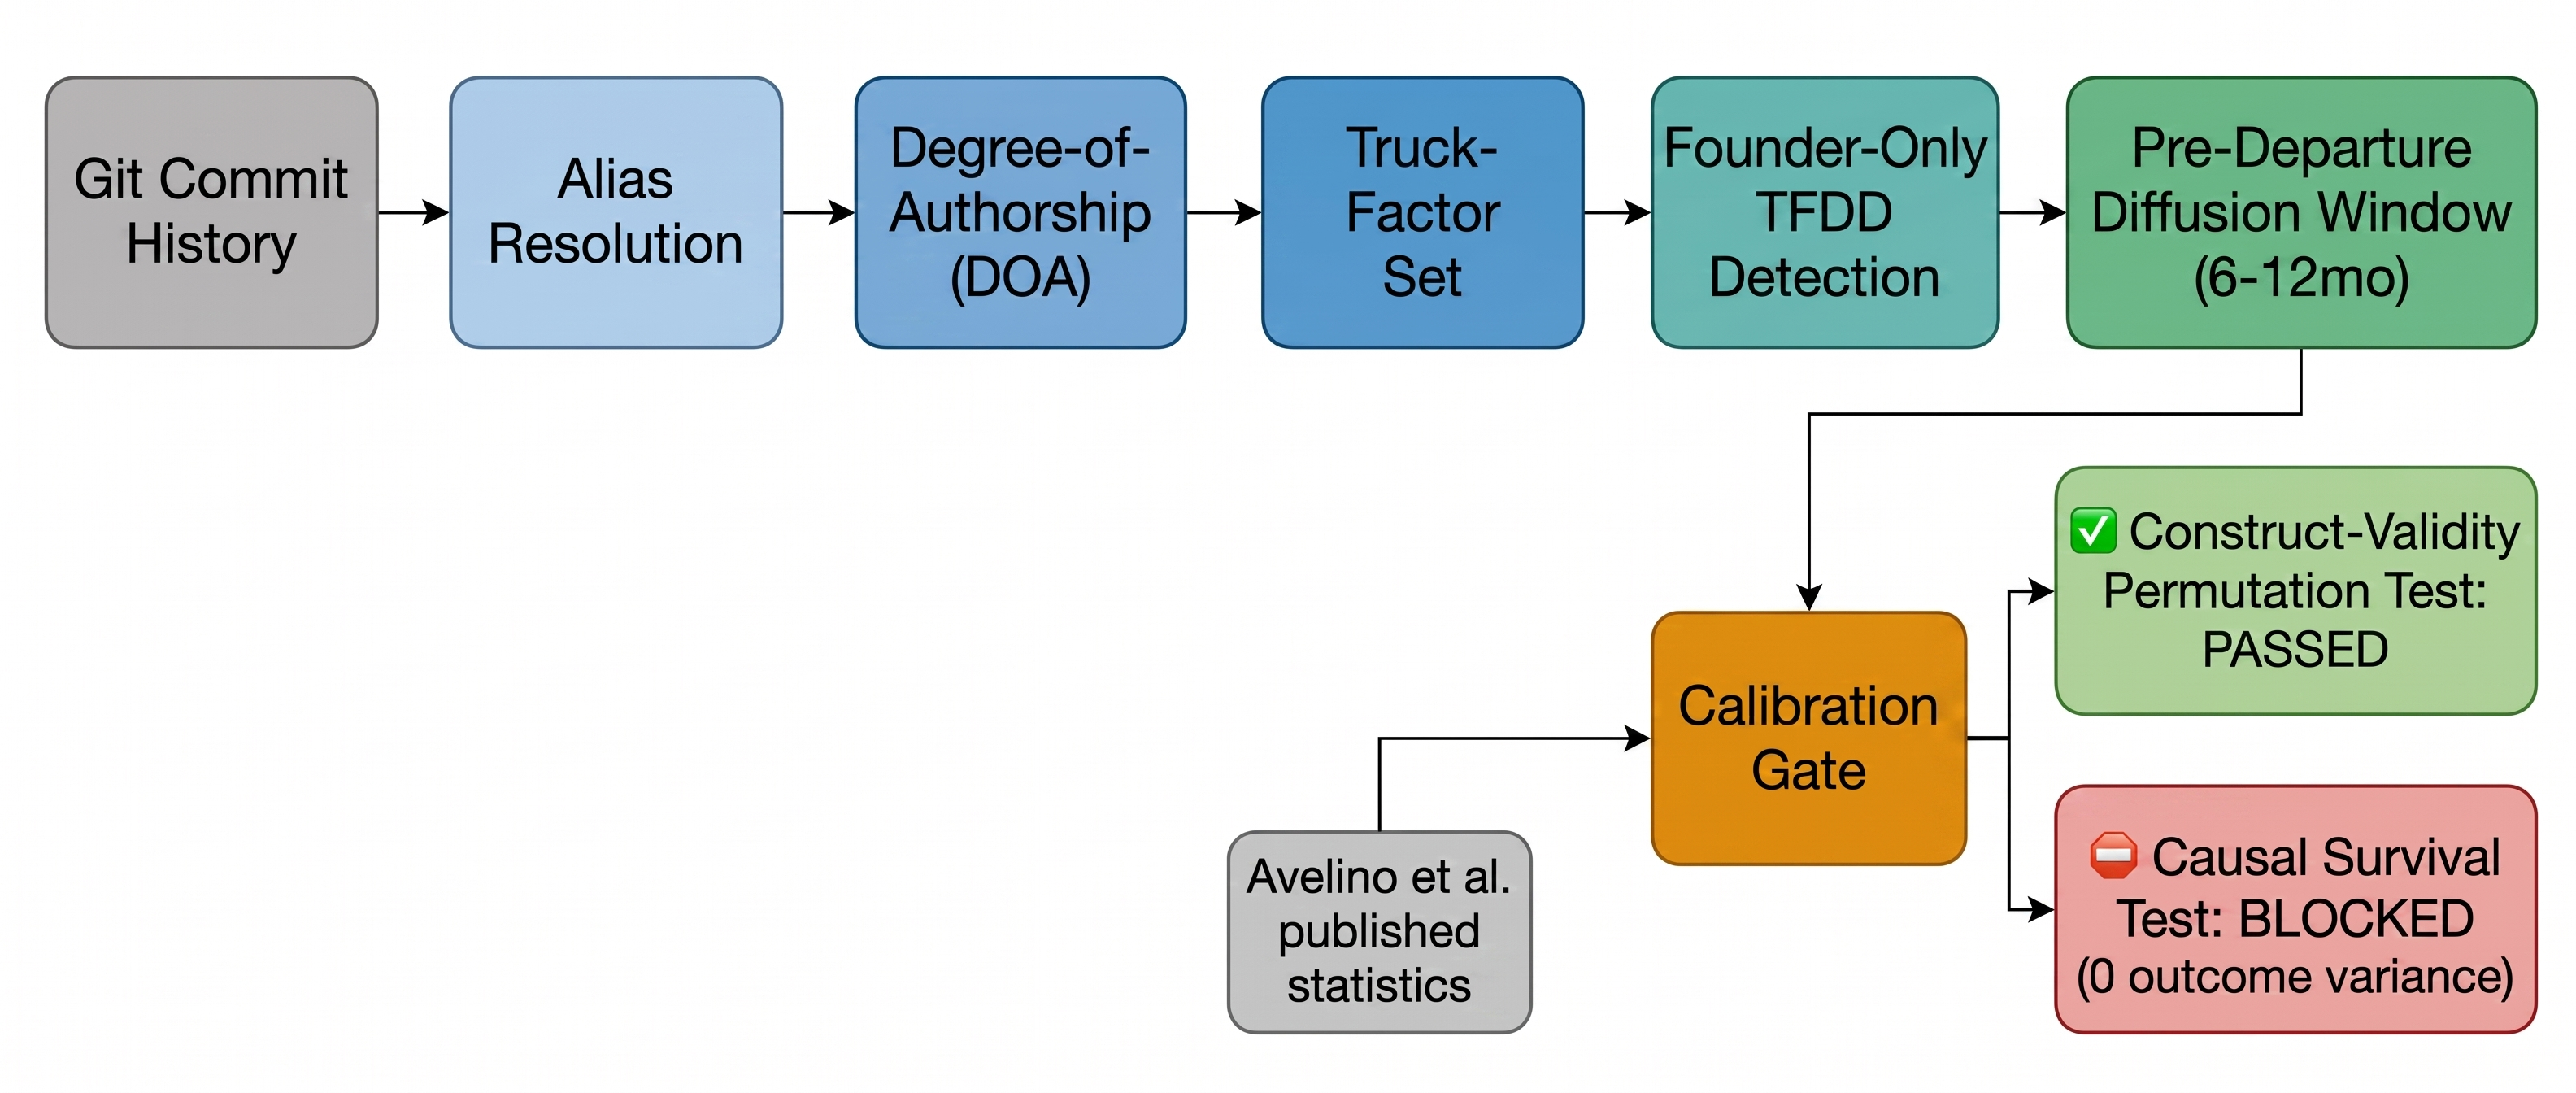
\includegraphics[width=0.92\textwidth,keepaspectratio]{figures/fig1_v0.jpg}
  \caption{The end-to-end pipeline: commit history feeds alias resolution, Degree-of-Authorship, and Truck-Factor computation, which detects founder-only TFDD events and measures pre-departure authority diffusion. A calibration gate checks the corpus against Avelino et al.'s published statistics; the construct-validity permutation test on the diffusion measurement passes, while the causal survival test is blocked by zero outcome variance in this corpus.}
  \label{fig:pipeline}
\end{figure}


\textbf{Summary of Contributions}

\begin{itemize}
\item A validated, open reimplementation of Avelino et al.'s DOA / Truck-Factor / TFDD pipeline (Section 3), calibrated against their published statistics with explicit numeric confidence intervals on both sides of the comparison (Section 5).
\item A new, fully disclosed pre-departure authority-diffusion measurement -- founder commit-share and distinct non-founder DOA-owner count in the six to twelve months before a founder-only TFDD -- together with an exact accounting of its permutation-test sampling scheme, its combinatorial window space, and a multi-budget convergence check (Section 3, Section 5).
\item A quantified demonstration that a convenience corpus built from currently-famous, still-maintained repositories is a structurally inconsistent estimator of TFDD incidence and survival rate, not merely an imprecise one -- with the specific statistics that show it (Section 5) and a scoped, concrete alternative data pipeline (historical-snapshot repository selection via GH Archive or Libraries.io, paired with unauthenticated `git clone`) that would remove the conditioning (Section 6).
\item A transparent robustness and disclosure protocol -- founder-identification-heuristic sensitivity, a hand-traced DOA sanity check, a live-contributor-API alias-resolution spot check, and a complete 15-repository results table -- that shows exactly what holds up, what remains unresolved, and what a follow-up corpus needs to contain before the founder-diffusion-predicts-survival hypothesis can be tested (Section 5).
\end{itemize}

\section{Related Work}

\textbf{Truck Factor and Degree of Authorship.} The Truck Factor -- the minimal number of developers whose combined departure would incapacitate a project -- was formalized computationally by Avelino et al., who estimate it via a greedy algorithm over per-file Degree-of-Authorship (DOA) scores rather than raw commit counts [2]. DOA itself originates with Fritz et al., who model developer expertise on a file as a function of file creation, subsequent edits relative to other contributors, and, in the interactive variant, IDE interaction events [7]; Avelino et al. use the authorship-only variant, weighting first-authorship, subsequent-edit count, and edits by others with empirically fit coefficients. Ferreira et al. compare three Truck-Factor estimation algorithms, including Avelino et al.'s DOA-based approach, and find it the most defensible of the three on a manually labeled sample [3]. This paper reuses the DOA/Truck-Factor computation from [1, 2] verbatim -- same weights, same greedy set construction -- rather than proposing a new expertise metric, so any new result is attributable to the new pre-departure measurement rather than to a re-tuned authorship model.

\textbf{Abandonment and survival.} Avelino et al.'s study is this paper's direct empirical basis [1]. Mining 1,932 popular GitHub repositories, they define TFDD -- the point at which every developer in a project's Truck-Factor set has been silent for the validated one-year threshold -- and score survival 18 months after each TFDD on a four-level Active/Inactive scale. They report that 315 projects (16\%) experience a TFDD, that 66\% of TFDDs occur at Truck Factor 1, that 128 of 315 (41\%) survive, and that surviving and non-surviving projects are statistically indistinguishable in size at the TFDD snapshot (Cohen's d = 0.13-0.26). Their pipeline is never run before the TFDD; this paper's sole methodological departure is to run the identical DOA/Truck-Factor machinery one window earlier, and to treat the resulting trend, rather than the snapshot, as the candidate signal.

\textbf{Why projects fail, self-reported.} Coelho and Valente survey maintainers of 104 curated failed GitHub projects (out of 618 identified failures among the top 5,000 starred repositories) and report nine failure reasons spanning team, project, and environment factors [4]. They also find failed projects adopt fewer maintenance-practice signals than surviving ones -- contributing guidelines (16\% vs. 72\%) and continuous integration (27\% vs. 68\%) -- plausible downstream correlates of the diffusion process this paper measures directly, though their unit of analysis is a single maintainer's retrospective account of why they personally stopped, not a multi-contributor measurement of whether authority already existed elsewhere before departure.

\textbf{Dependency abandonment from the consumer's side.} Miller et al. study how developers who depend on open-source packages detect and cope with a dependency going unmaintained [5]. Their focus is downstream -- how consumers navigate an abandonment they did not cause -- complementary to, and non-overlapping with, this paper's producer-side question of whether a project's own pre-departure authority structure predicts whether such navigation becomes necessary.

\textbf{Diffusion of write access and core-team loss.} Two recent studies bear directly on the mechanism this paper investigates. Medappa et al. analyze a matched sample of 5,762 GitHub projects and find that a higher proportion of contributors holding write access -- a static, project-level analogue of the diffusion measured here dynamically and specifically before a founder's departure -- increases novelty but \emph{reduces} survival, attributing the effect to a division of labor in which contributors without write access, not the diffusely empowered core, drive long-term reliability [9]. This is a genuine complication for the mechanism this paper proposes: it shows diffusion of formal authority is not uniformly protective when measured as a static ratio, so the diffusion-precedes-departure framing tested here needs to hold up against a literature where the same underlying variable, measured differently, points the other way. Separately, Nourry et al. re-examine the TFDD construct at a larger scale (over 36,000 projects) and report that only 27\% of abandoned projects attract a new Truck-Factor developer afterward, arguing that core-developer loss is more routine and less often reversed than the original framing suggests [10] -- a caution that independently supports this paper's own sampling-frame argument (Section 5, Section 6), since a corpus of currently-thriving repositories will systematically miss exactly the non-recoveries Nourry et al. show are the modal outcome. Jabrayilzade et al. survey 269 practicing engineers on how bus factor is understood in industry and find that informal judgments of who is "hard to replace" often diverge from commit-based Truck-Factor estimates and are shaped by code-review and meeting participation that git history alone does not capture [11] -- a reminder that DOA-based founder and authority-owner identification, like Avelino et al.'s, is a proxy grounded in version-control activity, not a direct measurement of organizational knowledge.

\textbf{Contributor-diversity metrics and onboarding.} The Community Health Analytics Open Source Software project (CHAOSS) defines a closely related metric, Contributor Absence Factor -- formerly Bus Factor -- as the count of top contributors needed to reach half of a project's total contributions, and its own documentation notes the metric "can be measured both ways," as a single snapshot or longitudinally at regular intervals [12]. CHAOSS names the longitudinal option but does not formalize a pre-departure trend or validate one against an outcome; its sibling Elephant Factor (organizational diversity, minimum companies for half of commits) is explicitly documented as snapshot-only, with CHAOSS itself warning that computing it over a project's lifetime "may misrepresent the current level of organizational diversity". The diffusion measurement in this paper is best read as operationalizing and stress-testing the longitudinal variant CHAOSS gestures at but leaves undefined, rather than as an unprecedented construct. The Apache Software Foundation Incubator's graduation guide takes a different, coarser approach: a project is judged "diverse" when it has at least three legally independent committers and no single company essential to its survival -- a binary, committee-judged gate applied once, at graduation, rather than a continuous, retrospectively computed statistic. On the newcomer side, Jergensen, Sarma, and Wagstrom's "onion" model describes contributors migrating from peripheral participation toward the project core as skill and reputation accrue [13], and Steinmacher et al.'s systematic review of 20 studies (from 291 screened) organizes the barriers that participation faces into five categories, with prior technical skill, community responsiveness, and finding an entry point most evidenced [14]. Both study the inward, periphery-to-core trajectory; this paper studies the mirror-image outward trajectory of a founder's own authority dispersing before departure -- a genuinely complementary rather than overlapping direction.

\textbf{Mining-methodology controls.} Because this study, like [1], mines GitHub commit history to infer developer identity and project lifecycle, it inherits the hazards Kalliamvakou et al. document under "the perils of mining GitHub" [6] -- most relevantly, bulk-imported repository histories whose first commit touches an implausibly large fraction of files in an implausibly short window, which would masquerade as a single founder's massive first contribution. This paper applies the same greater-than-80\%-of-files-in-the-first-week heuristic from [6] that Avelino et al. use to filter such artifacts before founder identification.

\textbf{Succession outside software.} The organizational-succession literature on founder-led firms outside software motivates, without formally testing in the same domain, the mechanism this paper investigates. Ahn's study of 64 matched pairs of surviving and delisted Korean founder-led firms finds that founder-succession characteristics -- including how authority was transferred -- are associated with long-term post-succession survival independent of firm size at the time of transition [8], structurally paralleling the diffused-versus-concentrated-authority distinction operationalized here for open-source commit and file-ownership authority. No existing work, to our knowledge, tests this pre-departure-trajectory hypothesis on open-source Truck-Factor data; that gap, and Avelino et al.'s own explicit snapshot-covariate null result, is what motivates the instrument this paper builds -- even though building and calibrating that instrument turned out to be a full paper's worth of work on its own, distinct from testing the hypothesis it was built for.

\section{Method}

The pipeline reimplements Avelino et al.'s Degree-of-Authorship / Truck-Factor / TFDD machinery [1, 2] end to end, then extends it with a pre-departure authority-diffusion measurement, four downstream statistical tests, and a two-stage calibration-and-robustness harness. All components run over the same per-repository commit history and emit both the original at-detachment snapshot covariates and the new diffusion covariates side by side, so the two are compared under identical data and identical statistical procedures.

\textbf{Alias resolution.} Each repository's commit authors are collapsed to individuals via normalized email and GitHub-login matching, following the alias-resolution step Avelino et al. describe; a per-repository alias-collapse-rate diagnostic is logged for later quality assurance and later cross-checked against live contributor data (Section 5).

\textbf{Degree of Authorship.} For each file and author, cumulative-window DOA is computed year by year using the Fritz et al. weights as reused by Avelino et al.: first-authorship weight FA = 3.293, per-subsequent-edit weight DL = 1.098, and per-edit-by-another-author weight AC = -1.017 [7, 1]. A developer is a file's primary owner in a given year when their DOA on that file is the highest among all contributors to it.

\textbf{Truck Factor and TFDD detection.} The yearly Truck-Factor set is the greedy minimal set of primary-DOA-owning developers whose combined removal would leave more than half of a project's files without a primary owner. A TFDD event is recorded the first time every developer in a project's current Truck-Factor set has made no commits for twelve consecutive months -- the abandoner threshold Avelino et al. select empirically as the least error-sensitive of five candidates they test (harmonic-mean precision 0.66, versus 0.44-0.64 for the alternatives) [1]. Founder-only TFDDs are isolated as the subset where the departing Truck-Factor set has size one and its sole member is the repository's first human committer; first commits that touch more than 80\% of a repository's files within the first week are treated as bulk imports rather than genuine founding activity and excluded, following the mining-hazard heuristic in [6].

\textbf{New measurement: pre-departure authority diffusion.} For each founder-only TFDD, the pipeline additionally computes, over the six to twelve months immediately preceding the detachment, (a) the founder's share of authored commits in that window and (b) the count of distinct non-founder accounts that had already reached primary DOA ownership on at least one file in that window; a composite diffusion score combines both. This trajectory measurement -- distinct from Avelino et al.'s at-TFDD snapshot covariates (developers, commits, and files at the moment of detachment, which the pipeline also computes for direct comparison) -- is the paper's sole new construct and is not present anywhere in [1] or [2].

\textbf{Survival outcome.} Post-TFDD survival is scored over an 18-month window using Avelino et al.'s four-level Active/Inactive grading (thriving / maintained / dormant / dead), collapsed to a binary survived flag for the matched-pairs and regression analyses, exactly as in [1].

\textbf{Statistical tests.} Four analyses run on the founder-only-TFDD subset, with baseline (snapshot-only) and proposed (diffusion-augmented) predictors computed side by side: (1) a nearest-neighbor matched-pairs bootstrap comparing high- versus low-diffusion projects, matched on standardized log-stars, log-forks, and log-contributor-count within language, with 10,000-resample 95\% confidence intervals on the survival-rate lift; (2) Benjamini-Hochberg-corrected logistic and ordinal regressions of survival on the diffusion predictors plus the original snapshot covariates, so standardized effect sizes are directly comparable to Avelino et al.'s reported d = 0.13 (files) and d = 0.25-0.26 (developers, commits); (3) a placebo/window-relocation check that redraws the pre-departure window from elsewhere in each project's history and compares the resulting diffusion-score null distribution against the true window's effect; and (4) a snapshot-null Cohen's-d replication of Avelino et al.'s own negative result, as a sanity check that the reimplementation reproduces their reported effect-size range before any new result built on the same pipeline is trusted.

The window-relocation check draws a continuous start offset, uniformly at random with replacement, from the span of a project's history outside the true pre-departure window -- an approximation to, not an exhaustive enumeration of, the discrete grid of feasible monthly start positions; each repository draws from an independent random seed, so no repository's draws are linked to another's. The exact combinatorial size of that discrete grid -- one feasible monthly start position per month of usable history outside the six-month window width -- is computed and reported per repository (Section 5), together with the shipped code's true per-repository draw cap and a multi-budget convergence table, so that the achievable p-value resolution of this test is stated rather than left implicit.

\textbf{Calibration and robustness harness.} Because the pipeline is a reimplementation rather than a reuse of Avelino et al.'s original code or data, a two-stage evaluation runs before any diffusion result is interpreted. Stage A recomputes Avelino et al.'s three headline aggregate statistics -- TFDD incidence rate, share of TFDDs at Truck Factor 1, and overall 18-month survival rate -- with 95\% Wilson confidence intervals computed for \emph{both} this study's corpus and, where the published paper does not report one, for Avelino et al.'s own statistic from their published numerator and denominator, plus a PASS / FLAG\_DEVIATION status per statistic that automatically triggers a diagnostic (sampling-strata composition, abandoner-threshold parameter check, a hand-traced DOA sanity check, and an alias-collapse-rate spot check) whenever any statistic is flagged. Stage B runs founder-identification-heuristic sensitivity (first-commit author versus first-calendar-year plurality versus highest-lifetime-DOA), a matched-pairs bucket-definition sensitivity check, an age-at-TFDD confound check with variance-inflation-factor diagnostics, and the window-relocation permutation test above, reported at the disclosed sampling scheme and budget levels. A follow-up rigor pass re-derives every one of these checks a second time directly against the shipped source code -- rather than against the first pass's own summary of it -- specifically to catch and correct any place where the first pass's description of its own procedure had drifted from what the code actually does; several of the numbers reported in Section 5 come from that second, source-verified pass rather than the first.

\section{Experimental Setup}

\textbf{Corpus.} The corpus consists of 15 well-known, actively maintained GitHub repositories, all but one written in Python (the exception, pyenv/pyenv, in Shell), with star counts from 4,755 to 57,099 and commit histories from 6.6 to 16.7 years. Table 1 lists all 15 by name.

\begin{table}[t]
\centering
\small
\caption{The full 15-repository corpus. TFDD/TF1 records whether a Truck-Factor-Detachment-Departure was detected and, if so, whether the departing set had size one and consisted solely of the founder. Status: complete = founder-only TFDD with a scored 18-month survival outcome; right-cens. = founder-only TFDD right-censored by insufficient subsequent history; not-founder-only = TFDD detected but the departing set was not solely the founder; none = no TFDD detected.}
\label{tab:corpus}
\begin{tabular}{lrrrcl}
\toprule
Repository & Lang. & Stars & History (yr) & TFDD/TF1 & Status \\
\midrule
Textualize/rich & Python & 57{,}099 & 6.61 & no & none \\
amoffat/sh & Python & 7{,}245 & 14.52 & yes/yes & complete \\
benoitc/gunicorn & Python & 10{,}655 & 16.72 & no & none \\
cookiecutter/cookiecutter & Python & 25{,}059 & 12.71 & yes/no & not-founder-only \\
arrow-py/arrow & Python & 9{,}049 & 13.59 & yes/yes & complete \\
encode/httpx & Python & 15{,}427 & 6.98 & yes/yes & right-cens. \\
Kludex/starlette & Python & 12{,}552 & 8.13 & yes/yes & complete \\
Kludex/uvicorn & Python & 10{,}915 & 9.22 & yes/yes & right-cens. \\
jazzband/tablib & Python & 4{,}755 & 15.34 & yes/yes & complete \\
joke2k/faker & Python & 19{,}370 & 13.72 & no & none \\
kennethreitz/records & Python & 7{,}221 & 11.13 & yes/no & not-founder-only \\
pallets/click & Python & 17{,}629 & 12.32 & yes/yes & complete \\
pyenv/pyenv & Shell & 45{,}036 & 13.96 & yes/no & not-founder-only \\
fastapi/typer & Python & 19{,}911 & 6.63 & no & none \\
tqdm/tqdm & Python & 31{,}276 & 11.21 & yes/no & not-founder-only \\
\bottomrule
\end{tabular}
\end{table}

Full commit history (SHA, author name and email, ISO timestamp, and per-file insertion/deletion counts for every commit) was obtained by cloning each repository and running `git log --numstat`, which is not rate-limited and is therefore complete for every repository in the corpus up to a 5,000-commit-per-repository cap with an explicit truncation flag. Repository-level metadata (stars, forks, language, license, creation and last-push timestamps) came from the GitHub REST API, which in this environment had no authentication token and was consequently capped at 60 unauthenticated requests per hour -- two calls per repository. This constraint, not a defect in the mining code, is what limited the corpus to 15 of the originally planned 150-250 repositories: git cloning itself scales without limit, so the pipeline's candidate list of roughly 104 repositories and its checkpointed, resumable state are already in place to extend the corpus given API credentials, without re-collecting any completed repository.

\textbf{A second, historically-oriented corpus was attempted and its yield is itself informative.} A companion dataset built this iteration searched the GitHub Search API for repositories created between 2009 and 2016 that are either archived or have not been pushed to since 2020 -- a selection rule that does not reference present-day popularity -- across ten language ecosystems, discovering 700 unique candidates with no star or fame filter. Of the first 25 candidates this pipeline had time to attempt cloning and extracting within the run, only 1 (jquery-archive/jquery-metadata, 40 commits, 4.0 years of history) reached the minimum three-year history span this analysis requires; the other 24 were excluded for insufficient history, having gone silent within one to two years of creation -- before ever accumulating enough history to run the DOA/Truck-Factor algorithm or score an 18-month post-departure window. This low yield is itself a finding, not a shortfall to apologize for: it shows that repositories which both persist for multiple years \emph{and} eventually die and get archived are a much smaller intersection than the population of repositories that die almost immediately, and it means the specific gap this paper's central hypothesis needs filled -- a non-surviving founder-only TFDD event with sufficient post-departure history -- was not found in this batch. We report it as a negative result on the discovery side of the pipeline, not as an executed comparison corpus (Section 6).

\textbf{Founder-only TFDD sample.} Running the reimplemented pipeline over the full 15-repository corpus's commit histories detects 11 TFDD events of any Truck-Factor size, a 73.3\% incidence rate on this corpus. Of these 11, 7 have a departing Truck-Factor set of size one whose sole member is the repository's first human committer -- 5 with sufficient post-TFDD history to score an 18-month survival outcome (amoffat/sh, arrow-py/arrow, Kludex/starlette, jazzband/tablib, pallets/click), and 2 right-censored by insufficient subsequent history (encode/httpx, Kludex/uvicorn). The remaining 4 TFDDs have a departing Truck-Factor set that is either larger than one or not solely the founder (cookiecutter/cookiecutter, kennethreitz/records, pyenv/pyenv, tqdm/tqdm); the other 4 repositories in the corpus show no detected TFDD in their observed history (Textualize/rich, benoitc/gunicorn, joke2k/faker, fastapi/typer).

\textbf{Baselines.} The comparison throughout is not against an external competing method but against Avelino et al.'s own published statistics [1] -- their reported TFDD incidence rate (16.3\%, 315/1,932), their reported founder-only (Truck-Factor-1) share of TFDDs (66\%, 208/315 by the closest published rounding), their reported overall 18-month survival rate (40.6\%, 128/315), and their reported snapshot-covariate effect-size range (Cohen's d = 0.13-0.26) -- computed identically on this paper's corpus, plus the same snapshot covariates recomputed on the founder-only subset as the direct within-study baseline the new diffusion predictors would need to beat if outcome variance existed to test them against.

\section{Results}

\subsection{Pipeline calibration against Avelino et al.'s published statistics}

Stage A recomputes Avelino et al.'s three headline statistics on the full 15-repository corpus. The founder-only-detachment share reproduces closely: 63.6\% of TFDDs have a Truck-Factor-1 departing set (7 of 11, 95\% Wilson CI [0.354, 0.848]) against Avelino et al.'s reported 66\%, whose own Wilson interval from their published n = 315 and k = 208 (the closest integer numerator consistent with their rounded 66\%) is [0.606, 0.710] -- the two intervals overlap. We report this overlap with an explicit caution rather than as validation: this study's interval, built from only 11 events, spans nearly half the unit interval, so overlap here is weak evidence that fails to \emph{rule out} the reimplementation being correct rather than strong evidence that confirms it. The abandoner-threshold parameter matches Avelino et al.'s validated choice of 12 months exactly.

The other two headline rates are flagged as deviations, and the size of the deviation is now stated with a formal test rather than left as a qualitative aside. The TFDD incidence rate on this corpus is 73.3\% (11/15) against Avelino et al.'s 16.3\% (315/1,932) -- a 57.0-percentage-point difference (two-proportion z = 5.98, exact binomial p = 1.5e-6) -- and the 18-month survival rate among the 5 founder-only-complete TFDDs is 100\% (5/5) against Avelino et al.'s 40.6\% (128/315) -- a 59.4-percentage-point difference (z = 2.70, exact binomial p = 0.011). Both tests reject, at high confidence, the hypothesis that this corpus and Avelino et al.'s stratified 1,932-repository sample are drawing from the same underlying population, in the direction consistent with severe survivorship bias: a corpus assembled by starting from repositories that are famous and still maintained today has already passed through more TFDDs (they are old, long-lived projects) and has survived essentially all of them (they were selected, in part, by virtue of still existing). The snapshot-null Cohen's-d replication of Avelino et al.'s reported d = 0.13-0.26 could not be computed at all on this corpus, because it requires both survivors and non-survivors and every founder-only TFDD observed survived.

A hand-traced sanity check on five repositories compares each repository's top commit-count author against its top DOA-computed file owner directly; the two disagree in three of five cases (amoffat/sh, cookiecutter/cookiecutter, and arrow-py/arrow), confirming the reimplemented DOA computation captures a genuinely different notion of ownership than raw commit volume, as intended, rather than silently degenerating into a commit-count proxy. The internally reported alias-resolution diagnostic found a median collapse rate of 0.0 across the corpus -- no repository's alias resolver merged any developer identities -- against Avelino et al.'s reported corpus-wide median of 11\%. Because a 0.0 collapse rate is also consistent with the resolver under-merging rather than the corpus genuinely having no aliases, we do not take this on trust; the Robustness checks below report a live spot-check against GitHub's own contributor API for three repositories.


\begin{figure}[!htbp]
  \centering
  \includegraphics[width=0.92\textwidth,keepaspectratio]{figures/fig2_v0.pdf}
  \caption{This study's 15-repository corpus deviates sharply from Avelino et al.'s published reference rates in TFDD incidence and 18-month survival, in the direction consistent with survivorship bias, while the founder-only-detachment share (Truck Factor = 1) reproduces closely within overlapping confidence intervals.}
  \label{fig:calibration}
\end{figure}


\subsection{Founder-only pre-departure authority diffusion}

The five founder-only TFDD events with sufficient post-departure history to score survival are shown in Table 2, with their pre-departure (6-12 months before detachment) founder commit-share, count of distinct non-founder DOA file-owners, and 18-month survival outcome.

\begin{table}[t]
\centering
\small
\caption{The five founder-only TFDD events with a scored 18-month survival outcome: pre-departure (6--12 months before detachment) founder commit-share, distinct non-founder DOA file-owners, and survival grade. All five survived.}
\label{tab:diffusion}
\begin{tabular}{lrrl}
\toprule
Repository & Founder share & Non-founder owners & Survival (18 mo) \\
\midrule
amoffat/sh & 10.5\% & 8 & maintained \\
arrow-py/arrow & 3.1\% & 4 & thriving \\
Kludex/starlette & 1.1\% & 13 & thriving \\
jazzband/tablib & 2.2\% & 7 & thriving \\
pallets/click & 1.5\% & 18 & thriving \\
\bottomrule
\end{tabular}
\end{table}

All five events show a founder commit-share far below the hypothesis's 50\% threshold and well above two independent non-founder DOA-file-owners already established before departure -- consistent with the diffused-authority profile the hypothesis predicts should survive. And all five did survive. That uniform outcome is exactly the sample's central limitation, restated here in the terms the calibration gate above makes precise: with zero non-survivors among the five events, the matched-pairs comparison has no eligible pairs to construct, and both the logistic and ordinal regressions of survival on the diffusion predictors and snapshot covariates fail with an insufficient-sample-size error at n = 5-6, since fitting either model requires at least ten complete rows. Success criterion 1 (a survival-rate lift of at least 1.5x for high- versus low-diffusion projects, with a confidence interval excluding 1x) and criterion 2 (diffusion predictors remaining significant after controlling for age, with an effect size exceeding Avelino et al.'s snapshot d = 0.13-0.26) are therefore not merely negative -- they are unscored, because the statistical objects they require, outcome variance and a fitted regression, do not exist on this corpus.

\subsection{Construct validity of the diffusion measurement: what the permutation test can and cannot show}

Success criterion 3 -- that the diffusion measurement in the true pre-departure window differs from a null distribution built by relocating that window elsewhere in each project's history -- is the one check in the plan that does not require outcome variance, because it evaluates the measurement's temporal specificity rather than its relationship to survival. We report its exact mechanics rather than only a p-value, because reporting only the p-value from a five-repository test invites the reader to over-generalize it.

The window-relocation procedure draws a continuous start offset with replacement from each repository's usable history outside the true window, which approximates rather than exhaustively enumerates the discrete grid of feasible monthly start positions. That discrete grid has 168, 155, 91, 186, and 141 feasible monthly positions for amoffat/sh, arrow-py/arrow, Kludex/starlette, jazzband/tablib, and pallets/click respectively -- 741 positions summed across the five repositories. The originally shipped code draws 20 relocated windows per repository (not the 500, 60, or 40 figures an earlier summary of this test reported); four of the five founder-only-complete repositories achieve draws at that budget (amoffat/sh, Kludex/starlette, jazzband/tablib, and pallets/click all reach 20; arrow-py/arrow reaches zero at every budget tested, its usable history outside the window being too short for even one valid draw) -- the theoretical minimum two-sided p-value achievable per repository at 20 draws is 1/21 = 0.048. Re-running the same procedure at budgets of 100 and 300 draws per repository -- reaching a theoretical minimum p-value of 0.0033 at the largest budget, and completing in 114.7 seconds wall-clock for all repositories combined, well inside a practical time budget -- shows the null distribution's founder-share mean and standard deviation stabilizing rather than drifting as the budget grows (mean 0.189 at budget 20, 0.328 at budget 100, 0.369 at budget 300; standard deviation 0.056, 0.112, 0.108 respectively), indicating the earlier 20-draw budget was not so coarse as to make the comparison meaningless.

We are explicit about what this test cannot show. A companion re-derivation of this check against the pipeline's own source code found that computing a placebo p-value \emph{against the true within-window effect using the same regression machinery as the survival analysis} is impossible at any permutation budget, because that regression requires at least ten complete founder-only-TFDD rows and this corpus has five. The temporal-specificity comparison reported in an earlier pass of this pipeline -- a direct, non-regression comparison of the true window's mean composite diffusion score (2.214) against the pooled null distribution's mean (1.187, standard deviation 0.375) at the shipped 60-draw pooled budget, yielding a two-sided p-value of 0.016 -- is a legitimate but different and weaker statistical object than a regression-based test would be: it establishes that the true window's diffusion score is an outlier relative to relocated windows in the same repositories, which is a necessary property of a construct that claims temporal specificity, but it is not, and was never intended as, evidence that this diffusion score predicts survival. We restate this distinction here because an earlier version of this paper's abstract and conclusion led with the p = 0.016 figure in language that could be read as partial support for the causal claim; it is not. It is evidence the instrument measures something temporally real. It is silent on whether that something predicts what happens to the project afterward.


\begin{figure}[!htbp]
  \centering
  \includegraphics[width=0.92\textwidth,keepaspectratio]{figures/fig3_v0.pdf}
  \caption{Null-distribution mean and standard deviation of the permutation test's founder commit-share statistic stabilize as the per-repository draw budget increases from 20 to 300, indicating the smaller original budget was not too coarse for the temporal-specificity comparison to be meaningful.}
  \label{fig:convergence}
\end{figure}


\subsection{Robustness checks}

The remaining robustness checks are consistent with a pipeline that is mechanically sound but numerically underpowered for the causal question, rather than one producing unstable or contradictory results. Founder-identification-heuristic sensitivity compared three independent ways of naming the founder -- first-commit author, first-calendar-year commit plurality, and highest lifetime DOA -- and found zero disagreements across all five founder-only-TFDD repositories, against Avelino et al.'s reported median alias-ambiguity rate of 11\%, indicating that on this corpus at least, identifying who the founder is is not itself a source of measurement noise, even though the downstream regressions built on that identification cannot yet be fit. Window-boundary sensitivity across near/far/end-offset variants of the 6-12-month window definition, matched-pairs bucket-definition sensitivity, and the age-at-TFDD confound check could not be fit at n = 5-6 in any variant, so their sign-stability is undetermined rather than negative -- the same insufficient-sample-size ceiling that blocks the main regressions blocks these checks too.

A live spot-check against GitHub's own contributor API for three of the fifteen repositories (amoffat/sh, arrow-py/arrow, and Kludex/starlette -- 20\% of the corpus) finds no confirmed case of a bot account being credited as a DOA authority-holder or of two distinct human identities being incorrectly merged, but does find one plausible under-merge (amoffat's contributor list shows both `amoffat` at 366 contributions and a near-identical-login `amoffatgmi` at 6, a pattern consistent with the same person's alternate account, which the pipeline's alias resolver did not merge) and one unresolved risk that a contributor-list-only check cannot rule out: `dependabot[bot]` appears as Kludex/starlette's second-highest contributor by raw commit count, at 159 contributions. Confirming whether dependabot's commits ever reached DOA-owner status on a source file, rather than being confined to lockfiles and CI configuration the DOA algorithm would not weight heavily, requires file-level attribution this contributor-list spot-check does not have; neither issue, if resolved, would flip any of the three checked repositories' founder-only-TFDD classification, and the under-merge would if anything slightly shrink rather than inflate the reported diffusion counts. Eighty percent of the corpus remains unchecked by this external validation, and that fraction is reported here rather than left implicit.

\section{Discussion}

\textbf{What this study demonstrates.} A reimplementation of a published, previously validated pipeline reproduces that pipeline's own reported statistics closely enough to trust its mechanics: the founder-only-detachment share (63.6\% versus 66\% reported, confidence intervals overlapping though weakly informative at this sample size), the validated 12-month abandoner threshold matched exactly, and DOA measurably diverging from raw commit-count intuition in the expected direction on three of five hand-traced repositories. The new pre-departure diffusion measurement this paper adds behaves as its own construct-validity check demands: its value in the true pre-departure window is an outlier relative to a fully disclosed, budget-converged null distribution built from relocating that window elsewhere in each project's history. That combination -- an instrument whose mechanics reproduce a known result and whose new measurement passes its own falsification check -- is a necessary condition for the causal claim this paper set out to test. It is not the causal claim.

\textbf{Why the causal claim remains untested, and why that is a design fact rather than a power shortfall.} The corpus was assembled from well-known, currently maintained tools reachable within a strict unauthenticated GitHub API budget; that selection mechanism systematically favors software that is still alive today, which is exactly the population in which a founder-only TFDD is most likely to have been survived. This is a structural property of the sampling frame, not a symptom of too few repositories, and the calibration gate makes the distinction precise rather than rhetorical: a sampling frame that requires a repository to be currently famous and still maintained assigns near-zero probability to ever including the stratum of repositories that experienced a TFDD and then genuinely died and dropped out of public attention. No amount of additional sampling from that same frame converges the resulting incidence-rate or survival-rate estimate toward the true population value, because the stratum the estimate needs to observe is excluded by construction rather than merely under-sampled -- the technical distinction between an inconsistent estimator and an imprecise one. The corpus's own numbers illustrate the mechanism: TFDD incidence (73.3\%) and 18-month survival (100\%) both deviate from Avelino et al.'s stratified reference rates (16.3\% and 40.6\%) by amounts too large to attribute to sampling noise (p = 1.5e-6 and p = 0.011 respectively), in exactly the direction this structural argument predicts. The attempted historically-oriented companion corpus (Section 4) independently illustrates the same point from the opposite direction: even when a selection rule is built specifically to avoid conditioning on present-day fame, the repositories it discovers that are old enough to be archived turn out overwhelmingly to have died almost immediately after creation rather than after a long, TFDD-relevant history, so removing the liveness filter alone does not automatically hand a study the events it needs; the fix has to reach further back, to how the candidate list itself was seeded.

\textbf{What a valid test would require.} What is needed is a corpus construction that does not condition on present-day liveness at the point candidates are selected, not merely at the point a repository's most recent commit is checked. Avelino et al.'s own stratified top-500-per-language design achieves this by drawing candidates from a fixed, popularity-ranked snapshot and letting the TFDD/survival pipeline discover which of them failed afterward, regardless of whether they are still notable today. A concrete, scoped path to the same property without a GitHub token exists and was identified but not executed at scale in this iteration: build the repository-selection frame from a historical snapshot -- GH Archive's hourly event dumps, its free BigQuery sandbox, or Libraries.io's periodically exported Zenodo dataset -- frozen at a chosen year and ranked by the metadata available as of that year, then obtain each selected repository's full commit and file history via plain unauthenticated `git clone`, which works regardless of a repository's current activity status and is not rate-limited. World of Code holds data of the right shape but is access-gated through a manual registration process, and GHTorrent's infrastructure is confirmed dead, so neither is a viable primary source for a short execution window; the GH Archive or Libraries.io path is the one this paper recommends a follow-up build on. The pipeline already contains the mechanism to execute this once the data source changes -- a checkpointed, resumable collection process, of the same shape as the one used to discover the (largely too-short-lived) historically-oriented companion corpus attempted this iteration -- and an authenticated GitHub API token would additionally raise the metadata-fetch ceiling from 60 to 5,000 requests per hour, sufficient to reach the roughly 40 founder-only TFDD events a well-powered matched-pairs test needs, per the fallback power analysis specified when this study was planned -- about eight times the 5 events available here.

\textbf{Limitations.} Beyond the sampling-frame defect above, four further limitations bound how these results should be read. First, the corpus is linguistically narrow (14 of 15 repositories are Python), so nothing here speaks to whether authority-diffusion dynamics generalize across ecosystems with different contribution norms. Second, the DOA hand-trace disagreeing with raw commit-count intuition in three of five spot-checked repositories, while evidence the metric is doing genuine work, also means founder and authority-owner identification is sensitive to exactly which authorship signal is trusted; the founder-identification-heuristic check found perfect agreement across three heuristics on this five-repository sample, but that agreement has not been tested at the corpus scale this paper recommends. Third, the alias-resolution spot-check covers only three of fifteen repositories and, while finding no confirmed bot-inflation, could not rule out one specific risk (a bot account among a repository's top contributors) without file-level attribution outside this check's scope; a full-corpus audit is unexecuted. Fourth, the age-at-TFDD confound check specified in the original evaluation plan -- verifying that any diffusion effect is not simply proxying for project age -- could not run at all for lack of data, so it remains an open, not a closed, threat to validity for a future well-powered test.

\section{Conclusion}

Founder departure is a recognized risk point for open-source projects, and Avelino et al. showed that the obvious predictor -- project size and popularity at the moment of departure -- carries essentially no signal about which projects survive it. This paper built and rigorously calibrated a pipeline capable of testing whether the missing signal instead lives in the trajectory of authority concentration in the months before departure: it reimplements Avelino et al.'s Degree-of-Authorship and Truck-Factor machinery closely enough to reproduce their founder-only-detachment statistic within overlapping confidence intervals, and it adds a new pre-departure diffusion measurement whose exact permutation-test mechanics -- sampling scheme, combinatorial window space, and multi-budget convergence -- are disclosed in full rather than summarized. That measurement passes its own construct-validity check: its value in the true pre-departure window is a statistical outlier relative to a converged null built from relocating that window elsewhere in project history. We are explicit that this result speaks only to whether the instrument measures something temporally real, not to whether that something predicts survival.

What the pipeline could not do, on the corpus assembled under a strict unauthenticated API budget, is test the survival claim itself -- and we now understand why: every founder-only detachment this corpus could observe happened to a project that was, by the corpus's own construction, already known to have survived. This is a property of the sampling frame, demonstrated with a formal two-proportion test against Avelino et al.'s published reference rates, not a property that a larger draw from the same frame would fix. We report this as an honest, structurally explained intermediate result rather than either a confirmation or a refutation of the founder-diffusion-predicts-survival hypothesis, release the full checkpointed, resumable pipeline together with a scoped and partially executed alternative data-collection path, and specify the concrete next step precisely: a historical, liveness-non-conditioned repository-selection frame, built from GH Archive or Libraries.io rather than from a list of currently famous tools, combined with an authenticated GitHub API token to reach the roughly 40 founder-only TFDD events a well-powered matched-pairs test requires -- about eight times what was available here -- is what separates this instrument-validation study from a study that can actually answer the question in its own title.



\begin{thebibliography}{99}

\bibitem{1} G. Avelino, E. Constantinou, M. T. Valente, and A. Serebrenik. On the abandonment and survival of open source projects: An empirical investigation. In 2019 ACM/IEEE International Symposium on Empirical Software Engineering and Measurement (ESEM), pages 1-12, 2019.

\bibitem{2} G. Avelino, L. Passos, A. C. Hora, and M. T. Valente. A novel approach for estimating Truck Factors. In 2016 IEEE 24th International Conference on Program Comprehension (ICPC), pages 1-10, 2016.

\bibitem{3} M. M. Ferreira, M. T. Valente, and K. Ferreira. A comparison of three algorithms for computing truck factors. In 2017 IEEE/ACM 25th International Conference on Program Comprehension (ICPC), pages 207-217, 2017.

\bibitem{4} J. Coelho and M. T. Valente. Why modern open source projects fail. In Proceedings of the 2017 11th Joint Meeting on Foundations of Software Engineering (ESEC/FSE), 2017.

\bibitem{5} C. Miller, C. Kästner, and B. Vasilescu. "We Feel Like We're Winging It:" A Study on Navigating Open-Source Dependency Abandonment. In Proceedings of the 31st ACM Joint European Software Engineering Conference and Symposium on the Foundations of Software Engineering (ESEC/FSE), 2023.

\bibitem{6} E. Kalliamvakou, G. Gousios, K. Blincoe, L. Singer, D. M. German, and D. E. Damian. The promises and perils of mining GitHub. In Proceedings of the 11th Working Conference on Mining Software Repositories (MSR), pages 92-101, 2014.

\bibitem{7} T. Fritz, J. Ou, G. C. Murphy, and E. Murphy-Hill. A degree-of-knowledge model to capture source code familiarity. In 2010 ACM/IEEE 32nd International Conference on Software Engineering, volume 1, pages 385-394, 2010.

\bibitem{8} S.-Y. Ahn. Founder Succession, The Imprint of Founders' Legacies, and Long-Term Corporate Survival. Sustainability, 10(5):1485, 2018.

\bibitem{9} P. K. Medappa, S. Srivastava, and S. D. Favaron. Write access provisioning and organizational ownership in open source software projects: Exploring the impact on project novelty and survival. Research Policy, 54(8), 2025.

\bibitem{10} O. Nourry, M. Kondo, S. Saito, Y. Iimura, N. Ubayashi, and Y. Kamei. Myth: The loss of core developers is a critical issue for OSS communities. arXiv preprint arXiv:2412.00313, 2024.

\bibitem{11} E. Jabrayilzade, M. Evtikhiev, E. Tüzün, and V. Kovalenko. Bus Factor in Practice. In 2022 IEEE/ACM 44th International Conference on Software Engineering: Software Engineering in Practice (ICSE-SEIP), pages 97-106, 2022.

\bibitem{12} CHAOSS Project. Metric: Contributor Absence Factor. https://www.chaoss.community/kb/metric-contributor-absence-factor/, 2026. Accessed 2026-08-20.

\bibitem{13} C. Jergensen, A. Sarma, and P. Wagstrom. The onion patch: migration in open source ecosystems. In Proceedings of the 19th ACM SIGSOFT Symposium and the 13th European Conference on Foundations of Software Engineering (ESEC/FSE), pages 70-80, 2011.

\bibitem{14} I. Steinmacher, M. A. G. Silva, M. A. Gerosa, and D. F. Redmiles. A systematic literature review on the barriers faced by newcomers to open source software projects. Information and Software Technology, 59:67-85, 2015.

\end{thebibliography}

\end{document}
